% 2.3.1.OldMethod.tex
%	Last update: 2020/02/19 F.Kanehori
%newpage
\subsubsection{従来の方法}
\label{subsubsec:OldMethod}
\parindent=0pt

Windows Visual Studioについて説明します。

\medskip
GitHubからSpringheadをダウンロードすると、
その中にライブラリをビルドするためのソリューションファイル
およびプロジェクトファイルが含まれています。

\Vskip{-.2\baselineskip}
\begin{narrow}[15pt]
	\begin{figure}[h]
	    \begin{center}
	    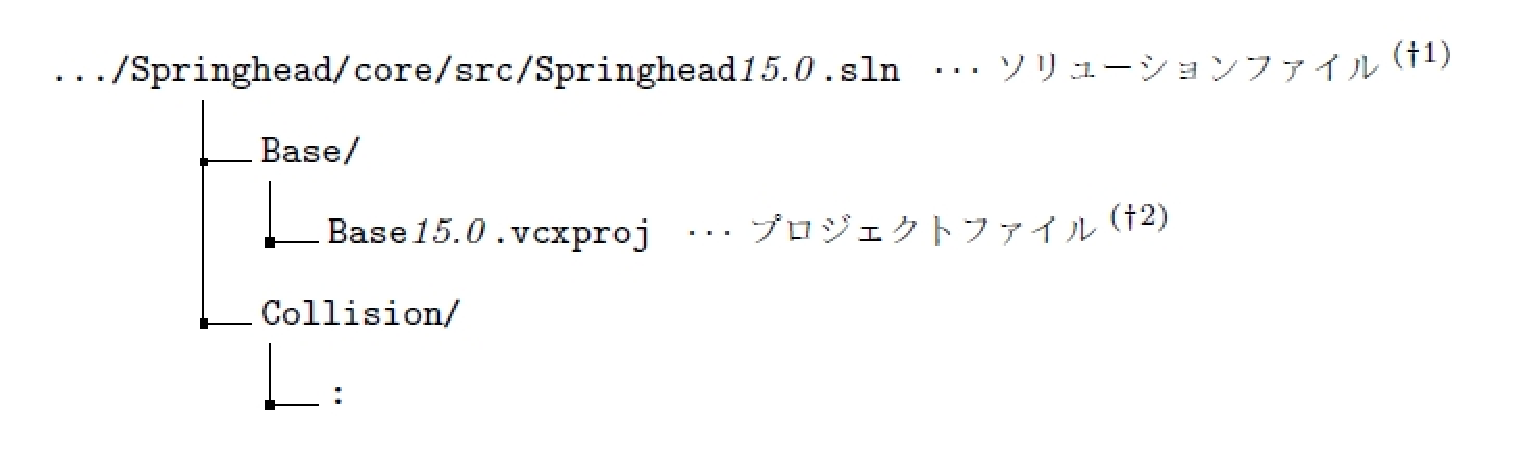
\includegraphics[width=.9\textwidth]{fig/DownloadTree.eps}
	    \end{center}
	    \label{fig:DownloadTree}
	\end{figure}
\end{narrow}
\Vskip{-.5\baselineskip}
%\begin{narrow}
%    \begin{narrow}[20pt]\begin{minipage}{\textwidth}
%	{\footnotesize{\dirtree{%
%		.1 \hspace{-10mm}C:/Springhead/core/src/Springhead\it{15.0}.sln
%			\Anno{\SolutionFile}.
%		.2 Base/.
%		.3 Base\it{15.0}.vcxproj
%			\Anno{\ProjectFile}.
%		.2 Collision/.
%		.3 :.
%	}}}
%	\medskip
%  \end{minipage}\end{narrow}
%\end{narrow}

上記の\SolutionFile を実行すればライブラリを生成することができ、
アプリケーションプログラム用のソリューションファイルに
上記の\ProjectFile を\KQuote{既存のプロジェクト}として追加すれば、
アプリケーションとライブラリの開発を同時に行なうことができました。

 後者の場合は、\ProjectFile は直接共有されることになります。このため、
\SprLib のソリューションとアプリケーション(複数でもよい)のソリューションとを
同時に開いて\ProjectFile に変更が及ぶような修正(ソースファイルの追加・削除)を
実施しても、
その変更はすべてのソリューションに直ちに反映されました。
(プロジェクトが環境外で変更された旨のダイアログが出ます)

\medskip
この方法はうまく機能していますが、次の点が難点として挙げられます。

\Vskip{-.5\baselineskip}
\begin{itemize}
  \item	Visual Studioのバージョンが変わる度に、
	ソリューションファイルとプロジェクトファイルを作り直す必要がある。
  \item	Windows以外のプラットフォームに対しては、
	Makefileなどを別途作成する必要がある。
\end{itemize}

% end: 2.3.1.OldMethod.tex
